\documentclass[11pt]{article}
\usepackage[utf8]{inputenc}
\usepackage{amsmath}
\usepackage{titlesec}
\usepackage{titling}
\usepackage{geometry}
\usepackage{media9}
\usepackage{graphicx}
\usepackage{hyperref}
\usepackage{fancyhdr}
\usepackage{wallpaper}
\usepackage{afterpage} 
\usepackage{pagecolor} 
\usepackage{multirow}
\usepackage{wrapfig}
\usepackage{lipsum} 
\usepackage{url}
\usepackage[toc,page]{appendix}
\usepackage{mdframed}
\usepackage{pgfgantt}
\usepackage{tabularx}


% Define colors
\usepackage{xcolor}
\definecolor{myblue}{RGB}{33, 66, 99}
\definecolor{mygray}{RGB}{169, 169, 169}
\definecolor{darkbluegrey}{RGB}{44, 62, 80} 

% Page styling
\pagestyle{fancy}
\fancyhf{}
\renewcommand{\headrulewidth}{0pt}
\renewcommand{\footrulewidth}{0pt}
\fancyfoot[C]{\thepage}
\renewcommand{\familydefault}{\sfdefault}

% Define a command for section headers
\titleformat{\section}
  {\color{myblue}\normalfont\Large\bfseries}
  {\color{myblue}\thesection}{1em}{}

% Define a command for subsection headers
\titleformat{\subsection}
  {\color{myblue}\normalfont\large\bfseries}
  {\color{myblue}\thesubsection}{1em}{}

% Adjust page margins
\geometry{a4paper, margin=1in}

% make references clickable
\hypersetup{
    colorlinks=true,
    linkcolor=blue,
    filecolor=magenta,      
    urlcolor=cyan,
}

\begin{document}

% Change the background color of the first page
\pagecolor{darkbluegrey}
\afterpage{\nopagecolor}

% Add a background image
\ThisCenterWallPaper{0.75}{./image/spike_brain.png}

\begin{titlepage}
  \vspace*{\stretch{1}}
  \begin{center}
    \textcolor{white}{\textbf{\Huge First Report}}\\ % changed text color to white
    \vspace{1cm}
    \textcolor{white}{\Large Sound Detection and Classification\\using Spiking Neural Networks} % changed text color to white
    \vspace{3cm}
  \end{center}
  \vspace*{\stretch{2}}
  \begin{center}
    \textcolor{white}{ % changed text color to white
      \textbf{COURREGE Téo}\\
      \textbf{GANDEEL Lo'aï}\\
      \vspace{1cm}
      \Large Date: \today}
  \end{center}
  \vspace*{\stretch{1}}
\end{titlepage}

\newpage

\tableofcontents

\pagebreak

\listoffigures

\pagebreak

\section{Introduction}

Our goal is to perform a thorough investigation and subsequent implementation of spiking neural networks (SNNs). SNNs, which are inspired by the neural signaling patterns of the human brain, show promising potential in various applications, especially in real-time processing and pattern recognition.

A spiking neural network (or SNN) is a type of artificial neural network that mimics the functionality of biological neural networks. Unlike traditional artificial neural networks (ANNs), SNNs incorporate the concept of time into their operating model. The neurons in SNNs generate spikes of activity and communicate through these spikes (like brain neurons stimulating each other with electrical impulses), allowing them to process information in a more complex and potentially more efficient manner.

This type of neural network theoretically consumes less energy than some ANNs and is potentially more efficient in terms of processing power (in practice, it will be necessary to create an adapted hardware architecture to take advantage of this potential). Therefore, it seems that the
Therefore, the use of this type of neural network could be a viable solution to a classification processing problem (especially in real time).

Our project will specifically address the challenges of applying SNNs to audio classification in the field of spiking neural network research. This report provides an overview of our initial progress in this area. Our project specifically addresses the problem of audio classification within the broader context of SNNs.

Before delving into the details, we outline key aspects including preprocessing, data manipulation/augmentation, initial model implementations, and a look at preliminary results.

Using audio data primarily from the \href{https://research.google.com/audioset/}{Google AudioSet} database, our work involves preprocessing, which includes converting signals to image representations, extracting features, and considering encoding schemes suitable for SNNs. Challenges related to data quality, context, and labeling complexity prompted the exploration of data augmentation strategies to improve model robustness.



In the following sections, we present the organizational structure of our project, the technical environment used, a detailed description of the work performed, the challenges faced, and the solutions implemented, concluding with a reflection on our achievements and future perspectives.


\pagebreak

\section{The project}

\subsection{Description of the project - Spiking Neural Networks}

Inspired by the neural signaling patterns of the human brain, SNNs introduce a temporal element into artificial neural networks. This temporal characteristic positions SNNs as promising candidates for real-time processing and pattern recognition tasks.

A spiking neural network is a variant of artificial neural networks designed to more closely mimic biological neural networks. Unlike traditional artificial neural networks (ANNs), which work with continuously changing time values, SNNs work with discrete events that occur at defined times. They take a set of spike values as input and produce a set of spike values as output.

The spiking behavior of a neuron in an SNN is modeled by a membrane potential equation. For example, in a leaky integrate-and-fire (LIF) neuron model, the membrane potential equation is defined by a set of parameters including a time constant ($\tau$), a resting potential ($u_{r1}$), a reset potential ($u_{r2}$), synaptic weights ($w_j$), and a firing threshold ($u_th$). The output spike ($s$) is determined based on the membrane potential ($u$) and various conditions. This discrete, event-based approach distinguishes SNNs from other types of neural networks.\cite{rething_comparison_ann_snn}

\begin{equation}
  \begin{cases}
    \tau \frac{d \: u(t)}{dt} = - [u(t) - u_{r_1}] + \sum_j w_j \sum_{t_j^k \in  S_i^{T_w}} K(t - t_j^k) \\
    \begin{cases}
      s(t) = 1 & u(t) = u_{r_2} \text{ if } u(t) \geq u_{th} \\
      s(t) = 0 & \text{otherwise}
    \end{cases}
  \end{cases}
  \label{eq:membrane_potential}
\end{equation}

This equation was first written as :
\begin{equation}
  \tau \frac{d \: u(t)}{dt} = - [u(t) - u_{r}] + RI
  \label{eq:lif_1}
\end{equation}

From a mathematical point of view, equation (\ref{eq:lif_1}) is a linear differential equation. Alternatively, an electrical engineer might recognize it as the equation of a leaky integrator or a $RC$ circuit with a parallel resistor ($R$) and capacitor ($C$). In neuroscience, this equation is called the passive membrane equation. \cite{neuronal_dynamics}

\begin{figure}[h]
  \centering
  \begin{minipage}{0.45\textwidth}
    \centering
    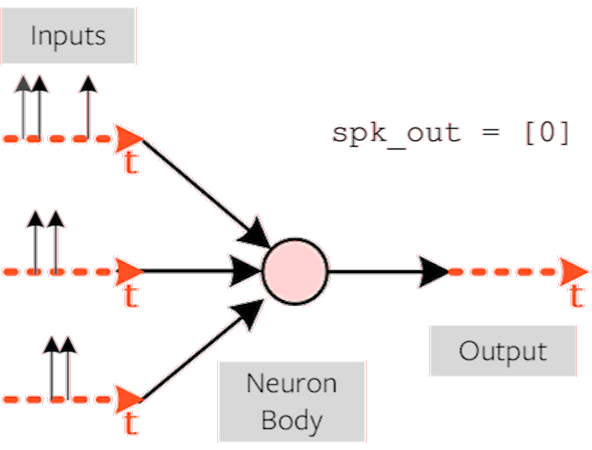
\includegraphics[width=1\textwidth]{image/def1.png}
    \caption{SNN input}
    \label{fig:def1}
  \end{minipage}\hfill
  \begin{minipage}{0.45\textwidth}
    \centering
    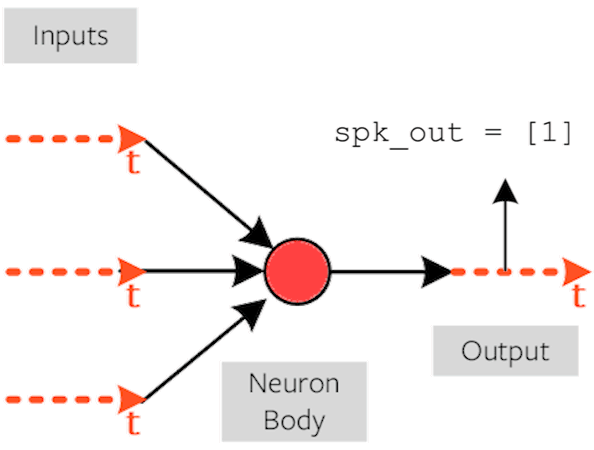
\includegraphics[width=1\textwidth]{image/def2.png}
    \caption{SNN output}
    \label{fig:def2}
  \end{minipage}
\end{figure}

\pagebreak

\subsubsection{Audio Classification Task}

Audio classification involves assigning a label to an audio clip based on its content. The audio classification task can be further divided into two subtasks: sound event detection (SED) and sound event classification (SEC). SED involves detecting the onset and offset times of sound events in an audio clip, while SEC involves assigning a label to each detected sound event.

In the context of audio classification, training an SNN involves working with image representations of audio data and encoding schemes suitable for SNNs.


\subsubsection{Project Objectives}

The primary goal of our project is to exploit the temporal processing capabilities of SNNs for audio classification tasks. Specifically, we want to develop models capable of classifying (and possibly detecting) sound events from audio data.

Furthermore, knowing that SNNs consume less power than traditional Artificial Neural Networks (ANNs), but have lower overall accuracy, we want to perform a performance comparison of SNNs with ANNs.

Achieving these goals would allow us to determine the potential of SNNs for audio classification tasks and identify the advantages and disadvantages of SNNs compared to other neural networks. It is also a great way for us to learn more about SNNs and audio classification.

\section{Organizing the project}

\subsection{Main tasks}

During the last full time period, we worked on:

\begin{itemize}
  \item \textbf{A preprocessing pipeline} that allows us to download, format, and segment the audio portion of the YouTube videos that make up the Google Audioset audio files into images.
        To be efficient, the pipeline needed to be parallelized.
  \item \textbf{Finding some correct data augmentation techniques} that can be used to improve the performance of the SNNs.
  \item \textbf{Finding a way to encode the audio data into spikes} that can be used as input for the SNNs.
\end{itemize}

\begin{itemize}
  \item \textbf{Implementing the SNNs} that will be used for the audio classification task.
        \subitem Training the SNNs on the audio data.
  \item \textbf{Implementing the ANNs}, which we would compare with the SNNs.
  \item \textbf{Comparing the performance of the SNNs and the ANNs} on the audio classification task.
\end{itemize}

\pagebreak

\subsection{Planning and team organization}

\subsubsection{Previous work - full time period}

\begin{figure}[h]
  \centering
  \resizebox{0.85\textwidth}{!}{
    \begin{ganttchart}[
        hgrid,
        vgrid,
        x unit=1.0cm,
        y unit title=0.7cm,
        y unit chart=0.9cm,
        title label font=\footnotesize,
        group label font=\footnotesize,
        milestone label font=\footnotesize,
        bar label font=\footnotesize,
        bar label node/.append style={align=left, text width=3cm}
      ]{1}{12}

      \gantttitle{Days}{12} \\
      \gantttitlelist{1,...,12}{1} \\

      \ganttgroup{\textbf{Setup and Literature Review}}{1}{1} \\

      \ganttgroup{\textbf{Working on the data}}{2}{6} \\
      \ganttbar[bar label node/.append style={align=left},
        bar/.append style={fill=red}]{Download, Format and Segment}{2}{5} \\
      \ganttbar[bar label node/.append style={align=left},
        bar/.append style={fill=blue}]{Data transformation}{2}{6} \\
      \ganttgroup{\textbf{Verification and SnnToch}}{6}{10} \\
      \ganttbar[bar label node/.append style={align=left},
        bar/.append style={fill=red}]{Data Verification and debugging}{6}{9} \\
      \ganttbar[bar label node/.append style={align=left},
        bar/.append style={fill=blue}]{Handling SnnTorch}{7}{10} \\

      \ganttgroup{\textbf{First implementations}}{11}{12} \\
      \ganttbar[bar label node/.append style={align=left},
        bar/.append style={fill=red}]{Testing ANNs}{11}{12} \\
      \ganttbar[bar label node/.append style={align=left},
        bar/.append style={fill=blue}]{Develop Spike Encoding}{11}{12} \\

    \end{ganttchart}
  }% Add this line
  \caption{Planning of the full time period}
  \label{fig:ftp1}
\end{figure}

\begin{itemize}
  \item Téo : \textcolor{blue}{blue}
  \item Loaï : \textcolor{red}{red}
\end{itemize}

So far, we have been able to encode and decode the audio data into spikes.

Since the first tasks we had to perform would not be connected until they were finished, we decided to work on them in parallel. This allowed us to be more efficient and, most importantly, to save time.

In the initial plan, there was no task related to data verification or debugging any part of the code. Each part of the preprocessing pipeline takes a lot of time to implement and test. We had to spend some time debugging the code and verifying the data.

\section{Work accomplished}

\subsection{Data}

Notes: In the section below, we decided not to include some code snippets because they were not very relevant to the report.

\subsubsection{The AudioSet}

In order to use the Google Audioset dataset, we needed to download the audio files and their associated labels. This first resulted in a file containing the links to the audio files and a file containing the label(s) of the audio files.
Their structure is as follows:

\begin{figure}[h]
  \centering
  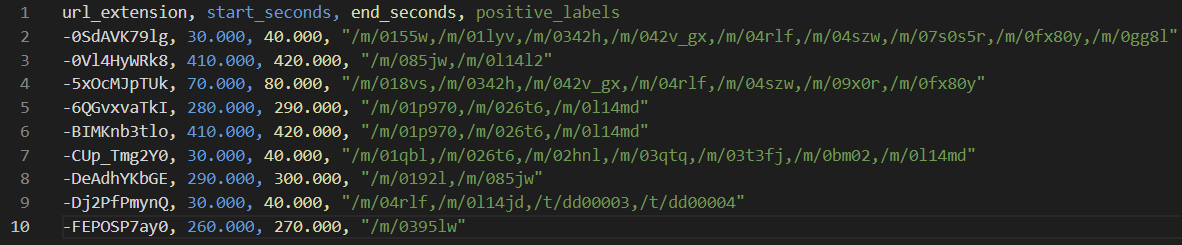
\includegraphics[width=\textwidth]{./image/structure_csv1.png}
  \caption{Structure and small content of the csv file containing the links to the audio files}
  \label{fig:structure_csv1}
\end{figure}

\subsubsection*{Filtering the data by labels}

The first column contains the links to the YouTube video, then the start and end time of the audio segment in the video, and finally the labels of the audio segment (there can be multiple labels for one audio segment).

Since we want to train our first model on small scenarios with only 3 classes \href{https://research.google.com/audioset/ontology/animal_1.html}{Animals}, \href{https://research.google.com/audioset/ontology/sounds_of_things_1.html}{Sound of things}, and \href{https://research.google.com/audioset/ontology/music_1.html}{Music}, we had to filter the data so that in all the rows that make up the csv file, there is at least one of the 3 classes we wanted to keep, but no repetition between the 3 classes.

Basically, we needed to iterate over the initial csv file to create 3 csv files, each containing only videos with one of the 3 classes we wanted to keep (see \texttt{reorder\_to\_categories.py}).

Also, there might be some repetitions between the labels associated with each audio segment, so we needed to remove those duplicates (see \texttt{reorder\_btw\_categories.py}).

(see our \href{https://github.com/LGPolytech/Project_S9}{GitHub repository}).

\subsubsection*{Downloading the audio files}

Once we had the csv files containing the links to the audio files, we needed to download them. To do this, we started using this \href{https://github.com/bakhtos/GoogleAudioSetScripts}{Github} repository as a base for our work. Since there were some problems using the \texttt{youtube-dl} library (that was changes to the \texttt{yt-dlp}), we had to modify the code to allow parallelization of the process (crucial for the efficiency of the pipeline if we don't want to wait for days to download the audio files).

We ended up with a code similar to the first one, but with some compatibility, performance and parallelization improvements (see \texttt{main\_dfs.py}).

\subsubsection*{Checking the data}

Once we had downloaded the audio files, we had to check that all the registered ones were not missing some information, corrupted or of duration less than 10 seconds (see \texttt{valid\_with\_labels}). This part ended-up being a source of problems as it consisted in a test and debug part.

\subsection{Study of SNNs}

\subsubsection{Neurons model}

Some frameworks have been created to modelize the dynamics of a neuron. Three of the models that have been created are the Leaky Integrate-and-Fire (LIF) Neuron Model (the most computationnally efficient), the Hodgkin-Huxley Neuron Model (the most biophysically pertinent), and the Izhikevich Neuron Model (a compromise between efficiency and realism).

\pagebreak

\begin{enumerate}
  \item  Leaky Integrate-and-Fire (LIF) Neuron:

        The LIF Neuron Model\cite{neuronal_dynamics} is a basic conceptualization of neurons as leaky integrators of incoming signals. The model is governed by a single differential equation which dictates the membrane potential evolution over time. It is the most used model in spiking neural networks.


        Equation:

        \begin{align*}
          \tau_m \frac{du}{dt} = -[u(t) - u_{\text{rest}}] + RI(t)
        \end{align*}

        \(\tau_m\): Membrane constant\\
        \(u\): Membrane potential\\
        \(u_{\text{rest}}\): Resting membrane potential\\
        \(R\): Membrane resistance\\
        \(I(t)\): Current\\


  \item Hodgkin-Huxley (HH) Neuron:


        The Hodgkin-Huxley Neuron model is the most biophysically realist, but is more complex. This model delves into the intricate details of neuronal behavior, incorporating ion channels and their conductances to mimic biological processes. This Model is built upon on a set of nonlinear differential equations.

        Equations:

        \begin{align*}
          C_m \frac{dV}{dt} & = -I_{\text{Na}} - I_{\text{K}} - I_{\text{L}} + I_{\text{ext}} \\
          I_{\text{Na}}     & = g_{\text{Na}} m^3 h (V - E_{\text{Na}})                       \\
          I_{\text{K}}      & = g_{\text{K}} n^4 (V - E_{\text{K}})                           \\
          I_{\text{L}}      & = g_{\text{L}} (V - E_{\text{L}})                               \\
          \frac{dm}{dt}     & = \alpha_m (1 - m) - \beta_m m                                  \\
          \frac{dh}{dt}     & = \alpha_h (1 - h) - \beta_h h                                  \\
          \frac{dn}{dt}     & = \alpha_n (1 - n) - \beta_n n                                  \\
        \end{align*}


        \begin{flushleft}
          \begin{description}
            \item[$C_m$:] Membrane capacitance
            \item[$V$:] Membrane potenti
            \item[$I_{\text{*}}$:] Sodium, Potassium, leakage, and external current
            \item[$g_{\text{*}}$:] Maximum sodium, potassium, and leakage conductance
            \item[$E_{\text{*}}$:] Nernst potential for sodium, potassium, and leakage (the equilibrium potential)
            \item[$m, h, n$:] Gating variables that represent the fraction of channels in the open state for sodium, potassium, and leakage channels, respectively
            \item[$\alpha_m, \beta_m, \alpha_h, \beta_h, \alpha_n, \beta_n$:] Voltage-dependent rate constants governing the kinetics of the opening and closing of ion channels
          \end{description}
        \end{flushleft}



  \item Izhikevich Neuron:

        The Izhikevich neuron model \cite{izhi_model} is a two-dimensional model designed to be as biologically plausible as the Hodgkin–Huxley model and as computationally efficient as the integrate-and-fire model. Depending on the parameters, the model reproduces spiking and bursting behavior of known types of neurons.

        Equations:

        \begin{align*}
          \frac{dv}{dt} & = 0.04v^2 + 5v + 140 - u + I_{\text{syn}} \\
          \frac{du}{dt} & = a(bv - u)
        \end{align*}


        $v$: Membrane potential

        $u$: Membrane recovery variable

        $a,ba,b$: Parameters determining the neuron's behavior

        $I_{\text{syn}}$: Synaptic current


        Although it is not the one which represents reality the most, LIF model is the best compromise if we take into account computation complexity.

        \begin{figure}[h]
          \centering
          \begin{minipage}{0.9\textwidth}
            \centering
            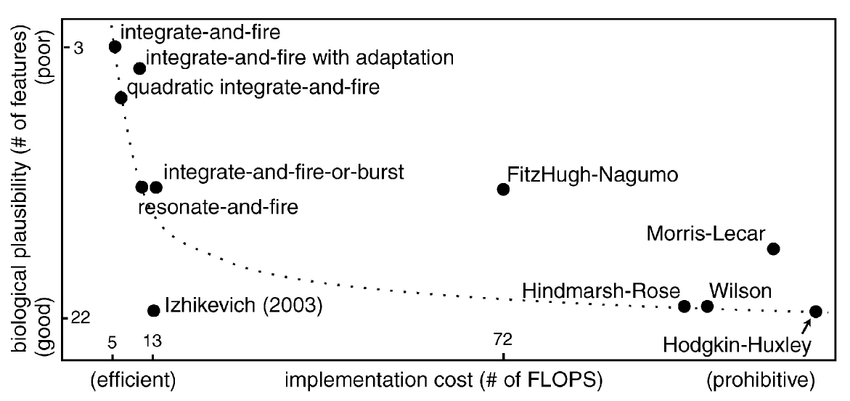
\includegraphics[width=1\textwidth]{"image/comparison_neuron.png"}
            \caption{Comparison of different neuron model's complexity and biological similarity}
            \label{fig:neuron_comparison}
          \end{minipage}\hfill
        \end{figure}
\end{enumerate}

\subsubsection{Spike encoding}

Encoding in SNNs refers to how information is represented and conveyed by the spikes of the SNN. In our study, we focus primarily on two of them:

\begin{itemize}
  \item Rate encoding:
        \subitem In rate encoding, information is represented by the firing rate of neurons. The more spikes a neuron produces in a given time window, the higher the firing rate and the stronger the encoded information.
  \item Latency coding:
        \subitem Temporal encoding focuses on the precise timing of spikes. The timing information of individual spikes is critical to the representation of the input data.
\end{itemize}

The exact timing of spikes can convey additional information, and the temporal patterns of spikes are used to encode features or events in the input signal.


\subsection{Spectrograms, Mel spectrograms, MFCC}


\subsubsection{Spectrograms}

Spectrograms are essential graphic tools in audio analysis. They offer a visual representation of the frequency spectrum of a sound signal as a function of time, providing detailed information on the frequency composition and temporal dynamics of an audio signal. This report explores the use of spectrograms in various contexts and highlights their importance in the analysis and understanding of audio signals.

A spectrogram is generated by applying a short-time Fourier transform (STFT) to an audio signal. This technique divides the signal into small time windows, then applies a Fourier transform to each window to obtain the frequency distribution at that particular moment. The results of these transformations are then represented graphically, using colors to indicate the intensity of frequencies at different periods.



\begin{figure}[h]
  \begin{equation}
    X_k = \sum_{n=0}^{N-1} x_n e^{-i 2 \pi k n / N}
    \label{eq:fourier_transform}
  \end{equation}
  \caption{Discrete Fourier Transform}
\end{figure}

Spectrograms enable in-depth analysis of the temporal characteristics of audio signals. Events such as transients, attacks and decays can be clearly identified, which is essential for understanding dynamic variations in music, speech and other forms of sound.

By examining the color and intensity of areas in a spectrogram, it's easy to identify the dominant frequencies present in an audio signal. This is particularly useful for detecting anomalies, characterizing musical instruments and separating sound sources.

Spectrograms are widely used in fields such as professional audio, music and linguistics. In particular, we are interested in Mel spectrograms, as well as MFCCs as input data for our neural networks.


\begin{figure}[h]
  \centering
  \begin{minipage}{0.9\textwidth}
    \centering
    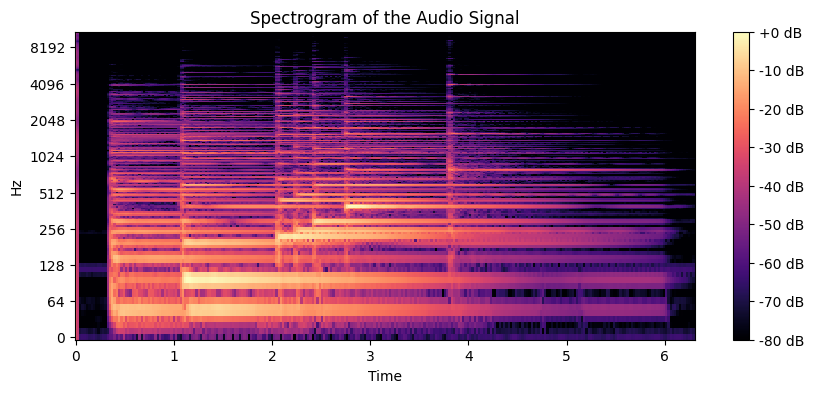
\includegraphics[width=1\textwidth]{"image/Spectrogram_piano.png"}
    \caption{Spectrogram of a slowly ascending piano arpeggio, we can notice the new notes with higher frequencies appearing over time, where the image is brighter}
    \label{fig:Spectrogram_piano}
  \end{minipage}\hfill
\end{figure}

\subsubsection{Mel Spectrograms}

While spectrograms offer a detailed view of the frequency spectrum of an audio signal, a significant evolution in audio analysis occurred with the introduction of Mel spectrograms.


These represent an adaptation of traditional spectrograms using a frequency scale based on the Mel scale, which is more in line with human auditory perception. This transition to Mel Spectrograms has broadened the possibilities of analysis, offering a more realistic representation of the auditory characteristics perceived by the human ear.


\begin{figure}[h]
  \centering
  \begin{minipage}{0.9\textwidth}
    \centering
    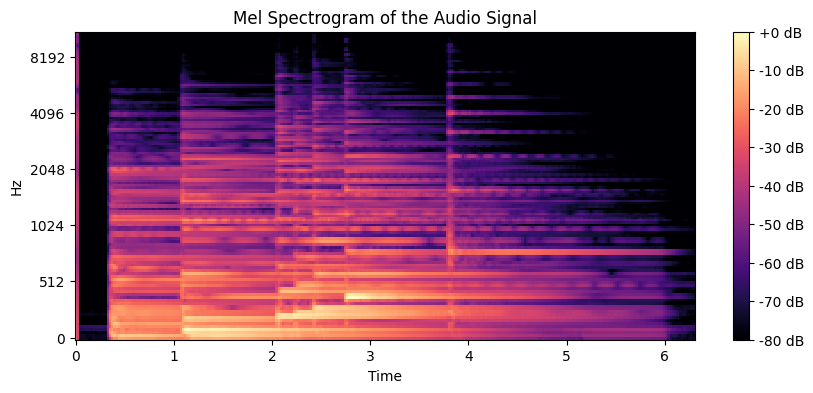
\includegraphics[width=1\textwidth]{"image/Mel_spectrogram_piano.png"}
    \caption{Mel Spectrogram}
    \label{fig:Mel_spectrogram_piano}
  \end{minipage}\hfill
\end{figure}

One of the main differences is that the bands corresponding to a note of the arpeggio are closer than in the spectrogram, which represents better the human auditory system


\subsubsection{Mel-frequency cepstral coefficients (MFCC)}

\href{https://en.wikipedia.org/wiki/Mel-frequency_cepstrum}{MFCCs} are derived directly from Mel spectrograms and are computed by applying a discrete cosine transform to the log power of Mel spectrograms. This approach captures information specific to human auditory characteristics while reducing data redundancy. MFCCs thus encapsulate frequency variations over time in a compact way, producing a set of cepstral coefficients that are widely used for automatic speech recognition and other audio signal processing tasks.

Two of the main advantages of MFCCs are compactness and information discrimination. MFCCs condense information while preserving the signal's distinctive characteristics. Compact representation facilitates storage, transmission, and processing of large amounts of data.
By focusing on perceptual features rather than raw frequency, MFCCs are less sensitive to pitch variations, improving the robustness of sound recognition.
The calculation of MFCCs involves several steps, including Mel scale transformation, calculation of the logarithm of spectral powers, discrete cosine transformation, and selection of relevant coefficients.


To summarize, to obtain an MFCC from an audio signal

\begin{itemize}
  \item Take the signal's Fourier transform (STFT).
  \item Map the powers of the resulting spectrum to the Mel scale, multiplying by overlapping window functions (triangular or cosine).
  \item Take the logarithm of the amplitudes at each mel frequency.
  \item Take the discrete cosine transform (DCT) of the list of logarithmic powers of the mel frequencies, as if it were a signal. The MFCCs are the amplitudes of the resulting spectrum.
\end{itemize}

\begin{figure}[h]
  \centering
  \begin{minipage}{0.75\textwidth}
    \centering
    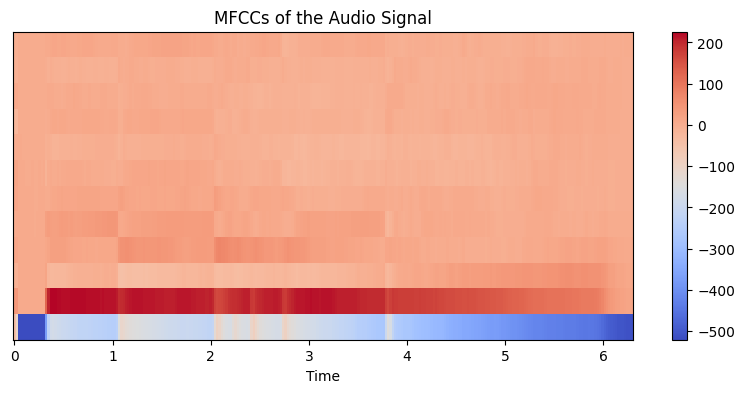
\includegraphics[width=1\textwidth]{"image/MFCC_piano.png"}
    \caption{MFCC}
    \label{fig:MFCC_piano}
  \end{minipage}\hfill
\end{figure}



\begin{equation}
  X_k = \sum_{n=0}^{N-1} x_n \cos \left[ \frac{\pi}{N} \left( n + \frac{1}{2} \right) k \right]
  \label{eq:dct}
\end{equation}



\subsection{Signal reconstruction}

To compare the most commonly used coding methods, we used a SNN neuron to encode and then decode MFCCs extracted from an audio signal. The two most commonly used coding approaches were compared: frequency coding and latency coding.

RESULTS: Reconstruction Quality

The results show that latency encoding (when normalized and linearized and with a sufficient number of time steps) leads to a better reconstruction quality of the audio signal than frequency encoding, which is much more subject to small errors that propagate during the reconstruction, errors due to the probability of emitting a pulse at each time step that does not perfectly represent the pixel intensity. This improvement can be explained by the ability of latency coding to capture fine temporal variations in the signal. However, due to the loss of information during signal transformation in MFCC, and more specifically in DCT, no reconstruction reaches the quality of the original signal.

In addition, with latency encoding, a pulse carries much more information, which can lead to less robustness in the face of noise, which can be very present in our dataset. We will therefore try to compare the two approaches in our SNN.

\begin{figure}[h]
  \centering
  \begin{minipage}{0.45\textwidth}
    \centering
    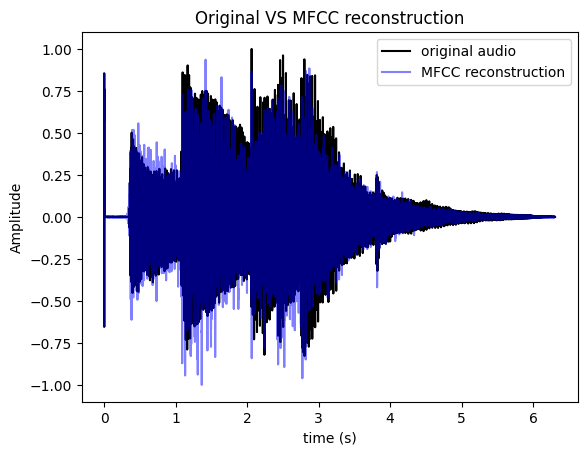
\includegraphics[width=1\textwidth]{"image/Original VS MFCC reconstruction.png"}
    \caption{Original VS MFCC reconstruction}
    \label{fig:OVSM}
  \end{minipage}\hfill
\end{figure}


\begin{figure}[h]
  \centering
  \begin{minipage}{0.45\textwidth}
    \centering
    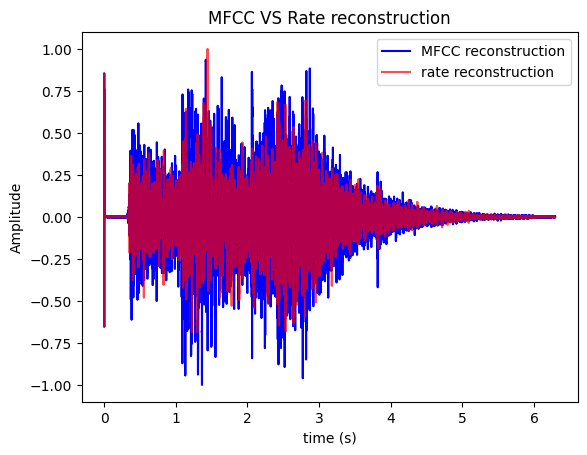
\includegraphics[width=1\textwidth]{"image/MFCC VS Rate reconstruction.png"}
    \caption{MFCC VS Rate reconstruction}
    \label{fig:MVSR}
  \end{minipage}\hfill
  \begin{minipage}{0.45\textwidth}
    \centering
    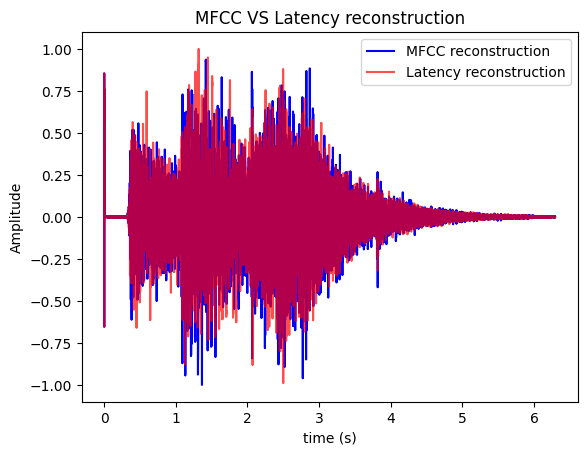
\includegraphics[width=1\textwidth]{"image/MFCC VS Latency reconstruction.png"}
    \caption{MFCC VS Latency reconstruction}
    \label{fig:MVSL}
  \end{minipage}
\end{figure}

\pagebreak

\section{Challenges and Solutions}
\textbf{Pipeline parallelization}

The first challenge we faced was the incompatibility of the \texttt{youtube-dl} library with the \texttt{ffmpeg} library, which can vary depending on the Python version you use.
For stability reasons, we decided to use the \texttt{yt-dlp} Python implementation instead of calling a shell command to perform operations (problems with the conda environment).

\textbf{Data Verification}

Another challenge was to verify the integrity of the data (not corrupted, no missing information, exactly 10 seconds long) and the download process (checking the existence of the audio url to download).

In addition, since we could not predict all possible outcomes that might occur, we had to go back and forth between data verification and data download to correct the problems that occurred (it took quite a while).

\textbf{Finding the relevant number of MFCCs features}

One of the issues was to find the relevant number of MFCCs features.

Increasing the number of MFCC coefficients increases the dimensionality of the feature vectors. While a higher dimensional feature space can capture more information, it also results in increased computational cost and memory requirements. Due to our limited resources, we had to find a compromise between the accuracy of the MFCC and the complexity.

It seems that the first few MFCC coefficients capture the most relevant information for audio processing (see \hyperref[fig:MFCC_piano]{figure 9}). These coefficients represent the signal's spectral envelope. As you go down the list of coefficients, they may contain less critical information and be more susceptible to noise.

The number of coefficients is also related to the diversity of our data; a more diverse dataset may require more coefficients as more features will be recognizable.

\textbf{Reconstruct the audio}

To reconstruct the audio, the data had to be properly normalized to create the MFCC and then denormalized to extract good audio. We used sklearn's \href{https://scikit-learn.org/stable/modules/generated/sklearn.preprocessing.MinMaxScaler.html}{MinMaxScaler} fitted to the data (which can apply both normalization and inverse normalization) to achieve our results.

\textbf{Latency encoding issues}

In latency encoding, there is a logarithmic dependence between input feature intensity and spiking timing, which can be problematic for reconstruction when the number of time steps is insufficient. To mitigate this problem, we applied a linear latency coding instead of a logarithmic one, and normalized it so that each spike occurs within our time steps.



\pagebreak

%\section{Conclusion et perspectives}

\section{Conclusion and Future Perspectives}

In conclusion, we have made some progress in the implementation of a data preprocessing pipeline, the theoretical study of SNNs, and the reconstruction of audio signals.
Our exploration of different data augmentation methods, neural models, and coding schemes gave us an insight into the possibilities and, most importantly, the challenges of SNNs in audio classification tasks.
Our study of signal reconstruction highlighted the trade-offs between frequency and latency coding. While latency coding showed promise in capturing fine temporal variations.
Comparing different encoding methods seems to be crucial for determining the most appropriate approach for our SNN-based audio classification.

This also gave us some lines of improvement:

\begin{enumerate}
  \item Combining our efforts to design, implement, and train SNN models.
  \item Implement SNN models for audio classification using the knowledge gained from our study.
  \item Compare different models of SNNs with different types of encoding.
  \item Complete the implementation of the existing ANN models.
  \item Perform performance evaluation.
\end{enumerate}

\pagebreak

\subsection*{Audio samples}
\begin{figure}[h]
  \centering
  \resizebox{0.8\textwidth}{!}{
    \begin{minipage}{.45\textwidth}
      \centering
      \includemedia[
        width=\textwidth,
        addresource=audio/piano_original.wav,
        flashvars={
            source=audio/piano_original.wav
            &autoPlay=false
            &hideBar=false
          },
      ]{\fbox{Play}}{APlayer.swf}
      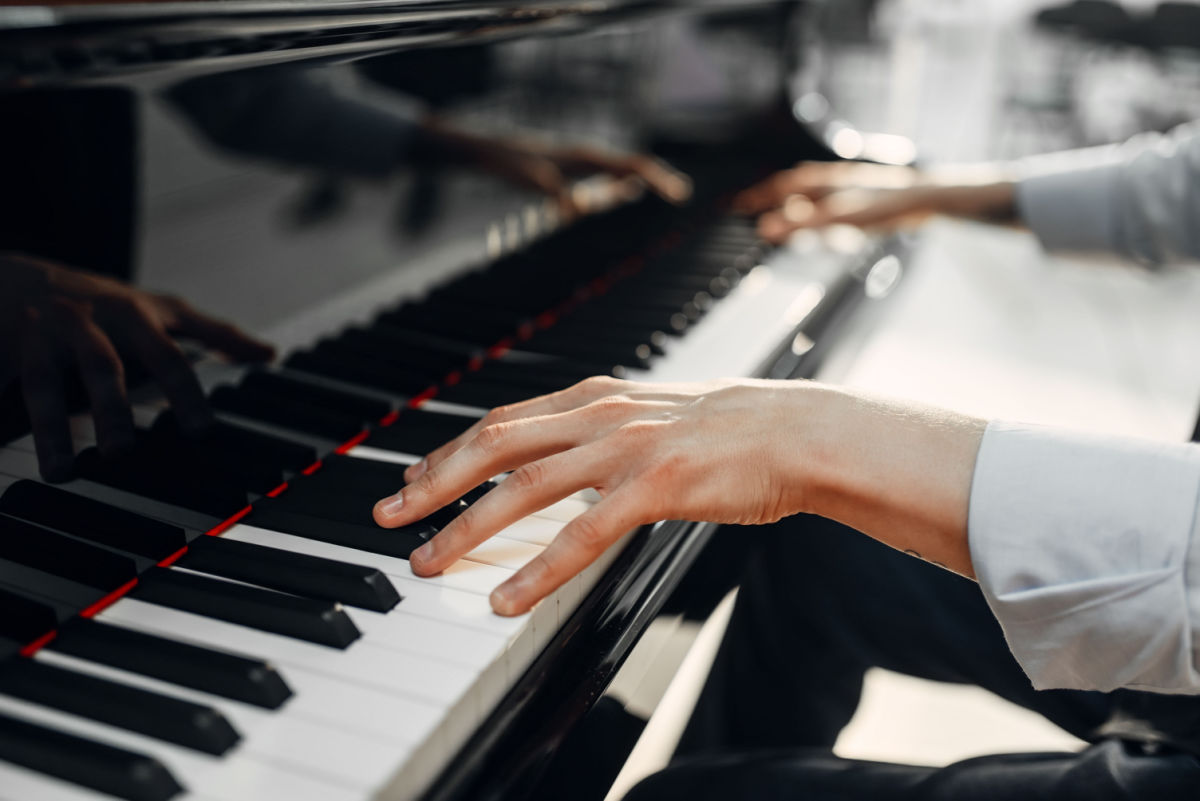
\includegraphics[width=\textwidth]{image/piano.png}
      \caption{Original Audio}
    \end{minipage}
    \begin{minipage}{.45\textwidth}
      \centering
      \includemedia[
        width=\textwidth,
        addresource=audio/piano_mfcc_reconstruction.wav,
        flashvars={
            source=audio/piano_mfcc_reconstruction.wav
            &autoPlay=false
            &hideBar=false
          },
      ]{\fbox{Play}}{APlayer.swf}
      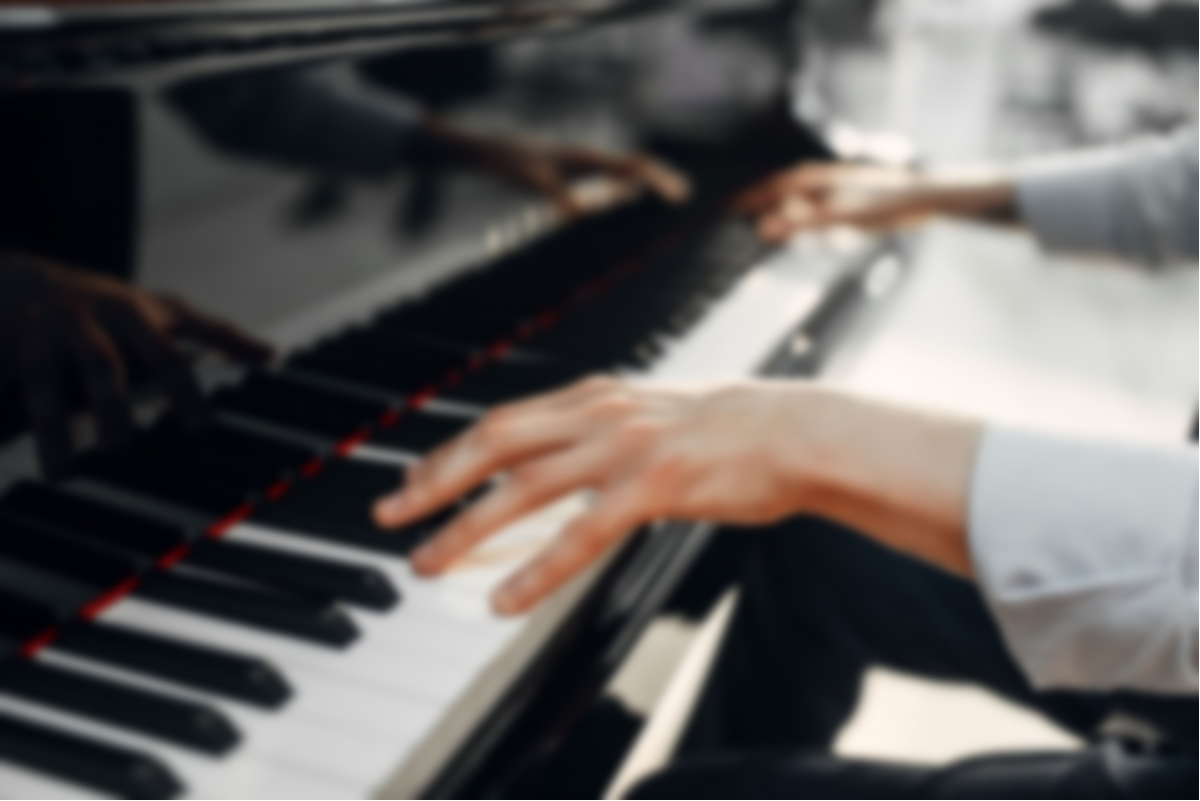
\includegraphics[width=\textwidth]{image/piano_blur1.png}
      \caption{MFCC Reconstruction}
    \end{minipage}
  }
\end{figure}

\begin{figure}[h]
  \centering
  \resizebox{0.8\textwidth}{!}{
    \begin{minipage}{.45\textwidth}
      \centering
      \includemedia[
        width=\textwidth,
        addresource=audio/piano_latency_reconstruction.wav,
        flashvars={
            source=audio/piano_latency_reconstruction.wav
            &autoPlay=false
            &hideBar=false
          },
      ]{\fbox{Play}}{APlayer.swf}
      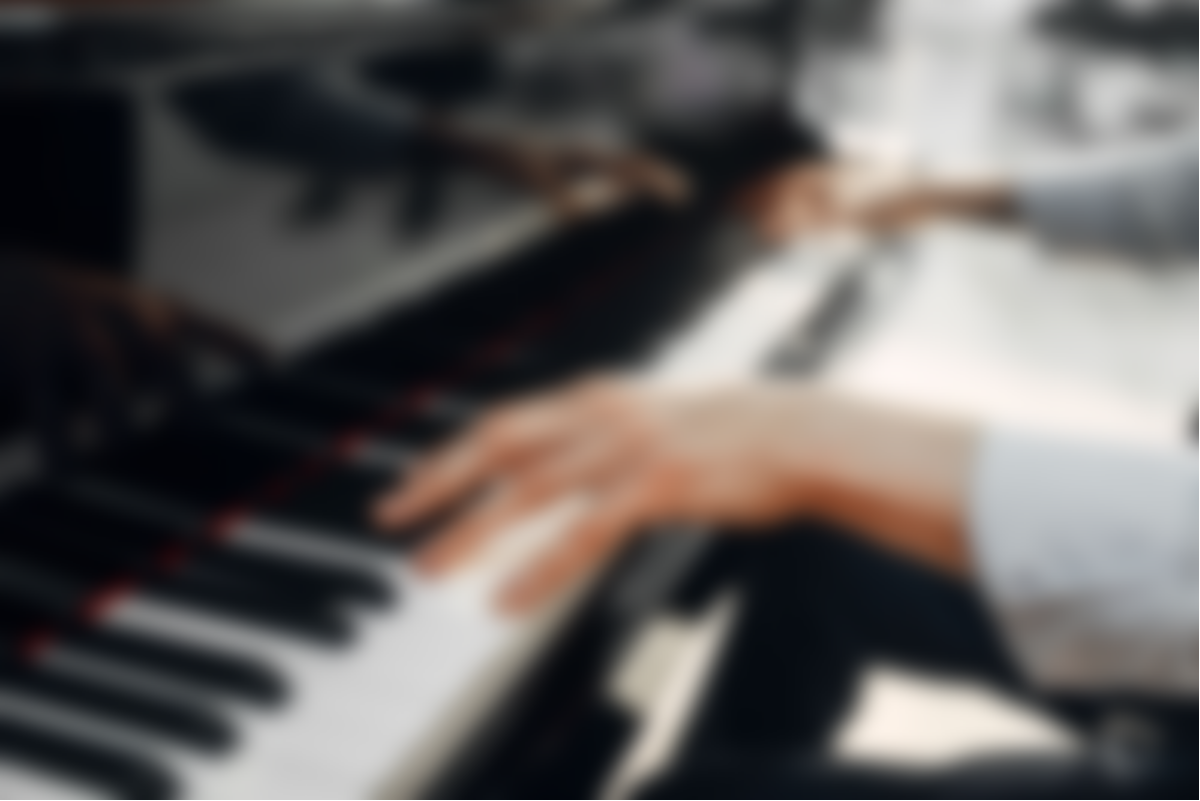
\includegraphics[width=\textwidth]{image/piano_blur2.png}
      \caption{Latency Reconstruction}
    \end{minipage}
    \begin{minipage}{.45\textwidth}
      \centering
      \includemedia[
        width=\textwidth,
        addresource=audio/piano_rate_reconstruction.wav,
        flashvars={
            source=audio/piano_rate_reconstruction.wav
            &autoPlay=false
            &hideBar=false
          },
      ]{\fbox{Play}}{APlayer.swf}
      
\includegraphics[width=\textwidth]{image/piano_blur3.png}
      \caption{Rate Reconstruction}
    \end{minipage}
  }
\end{figure}

\pagebreak

\section{Technical environment}

\subsection{Computational tools}

We worked on our personal computers and we used the following computational tools:


\begin{figure}[h]
  \begin{center}
    \begin{tabularx}{\textwidth}{|X|X|}
      \hline
      \textbf{Softwares}  & \href{https://code.visualstudio.com/}{Visual Studio Code}     \\
                          & \href{https://jupyter.org/}{Jupyter Notebook}                 \\
                          & \href{https://git-scm.com/}{Git}                              \\
                          & \href{https://github.com/}{Github}                            \\
                          & \href{https://colab.research.google.com/}{Google Colab}       \\
                          & \href{https://www.anaconda.com/products/individual}{Anaconda} \\
                          & \href{https://www.overleaf.com/}{Overleaf}                    \\
      \hline
      \textbf{Programming languages}
                          & \href{https://www.python.org/}{Python}                        \\
                          & \href{https://www.latex-project.org/}{Latex}                  \\
      \hline
      \textbf{Libraries}  & \href{https://pytorch.org/}{Pytorch}                          \\
                          & \href{https://librosa.org/doc/latest/index.html}{Librosa}     \\
                          & \href{https://numpy.org/}{Numpy}                              \\
                          & \href{https://pandas.pydata.org/}{Pandas}                     \\
                          & \href{https://matplotlib.org/}{Matplotlib}                    \\
                          & \href{https://pysox.readthedocs.io/en/latest/}{sox}           \\
                          & \href{https://github.com/ytdl-org/youtube-dl}{Youtube-dl}     \\
      \hline
      \textbf{Frameworks} & \href{https://github.com/eriksoper/SnnTorch}{SnnTorch}        \\
      \hline
    \end{tabularx}
  \end{center}
  \caption{Computational tools}
\end{figure}

\href{https://github.com/LGPolytech/Project_S9}{(Our Github repository)}

\pagebreak

% Bibliography
\bibliographystyle{siam}
\bibliography{ref}

\end{document}